\input{../header}
\hyphenpenalty=5000

\rhead{Your name: \rule{8cm}{0.15mm}}

\begin{document}

\everymath{\displaystyle}

\section{Learning target D2, version 1}

D2: Express real world situations as differential equations, determine any equilibrium solutions, and explain the significance of the equilibrium solutions in context.

\hrulefill

A population of flamingos changes over time according to the differential equation 
\[\dfrac{dP}{dt} = -\frac{1}{3}\, P\, (1-P)(5-P),\]
where $P$ is measured in thousands (and $t$ is probably measured in months or years).

Draw a phase graph and a slope field. Find all the equilibrium solutions, and explain how you know each one is stable or unstable.
 
\begin{center}
	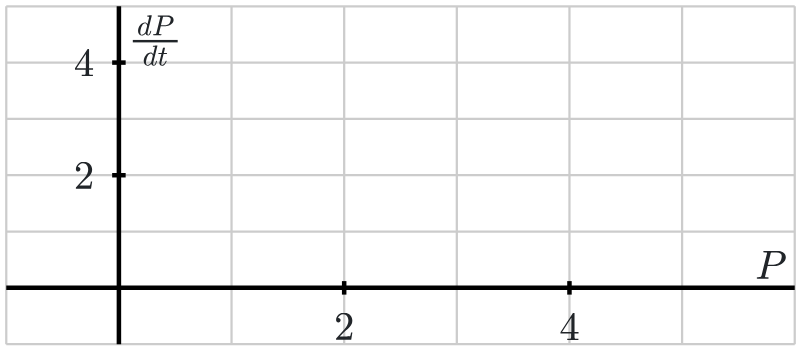
\includegraphics[width=0.75\textwidth]{../images/d2-phase-graph-axes.png}

	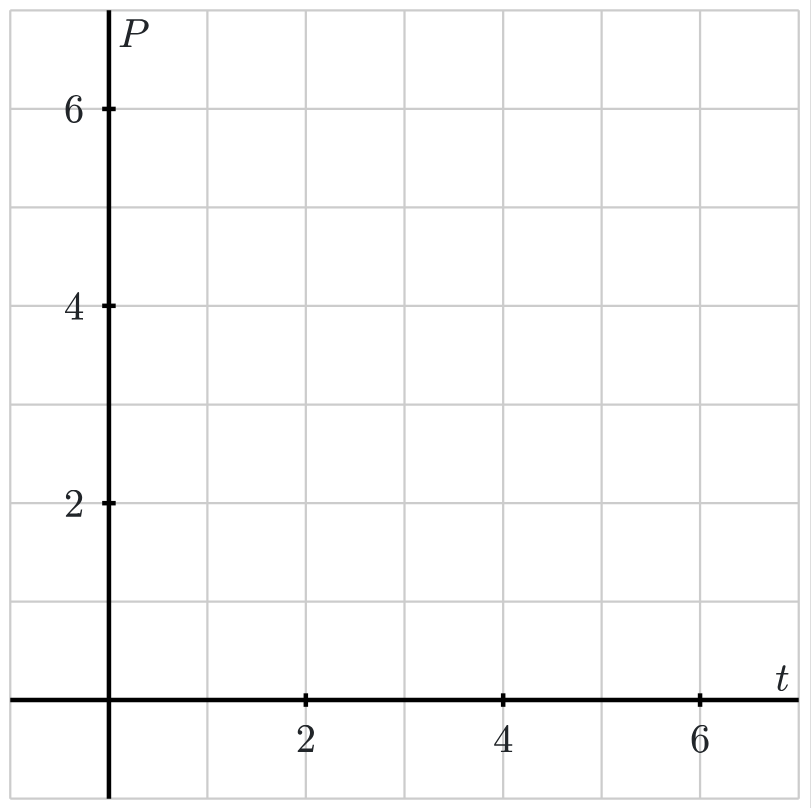
\includegraphics[width=0.7\textwidth]{../images/d2-slope-field.png}
\end{center}
%%%%%%%%%%%%%%%%%%%%%%%%%%%%%%%%%%%%%%%%%%%%%%%%%%%%%%%
\pagebreak
%%%%%%%%%%%%%%%%%%%%%%%%%%%%%%%%%%%%%%%%%%%%%%%%%%%%%%%

\section{Learning target D2, version 2}

D2: Express real world situations as differential equations, determine any equilibrium solutions, and explain the significance of the equilibrium solutions in context.

\hrulefill

Newton's law of cooling says that a hot object cools\footnote{Or a cold object warms!} at a rate proportional to the difference between its current temperature and the ambient temperature, which let's say is 73 degrees:
\[\dfrac{dT}{dt} = -k\cdot(T-73)\]

Draw a slope field (on $T$ vs. $t$ axes), a phase graph (on $\tfrac{dT}{dt}$ vs. $T$ axes), or work in other ways to:
\begin{itemize}
	\item figure out any equilibrium solution(s),
	\item classify the stability of any equilibrium solution(s),
	\item and explain why the equilibrium solution(s) make real-life sense.
\end{itemize}

\end{document}